\subsubsection{ΠΕΡΙΠΤΩΣΗ ΧΡΗΣΗΣ 1: Αναζήτηση από Απλό Χρήστη-Παρατηρητή }
\subsubsubsection{Χρήστες (ρόλοι) που εμπλέκονται}
Στη συγκεκριμένη περίπτωση χρήσης υπάρχει ουσιαστικά μόνο ο Απλός Χρήστης-Παρατηρητής, ο οποίος εισέρχεται στη σελίδα προκειμένου να παρατηρήσει τις πλέον πρόσφατες τιμές των πρατηρίων υγρών καυσίμων στην περιοχή που επιθυμεί.
\subsubsubsection{Προϋποθέσεις εκτέλεσης}
Οι συνθήκες οι οποίες πρέπει να ισχύουν είναι οι εξής: 
\begin{enumerate}
	\item Σύνδεση στο διαδίκτυο
	\item Η βάση δεδομένων του backend είναι online
	\item Η διαδικτυακή διεπαφή λειτουργεί
	\item Η διεπαφή με το API του MapBox είναι ενεργή
\end{enumerate}
\subsubsubsection{Περιβάλλον εκτέλεσης}
Το περιβάλλον στο οποίο εκτελείται η περίπτωση χρήσης είναι η διαδικτυακή διεπαφή χρήστη, είτε από κάποιο φυλλομετρητή, είτε από κάποιο smartphone.
\subsubsubsection{Δεδομένα εισόδου}
Δεν υπάρχουν δεδομένα εισόδου τύπου log-in, μιας και ο απλός χρήστης-παρατηρητής δε χρειάζεται να συνδεθεί. Ωστόσο, μπορούμε να θεωρήσουμε σαν δεδομένο εισόδου τη γεωγραφική τοποθεσία του απλού χρήστη-παρατη-ρητή που παραχωρείται στο σύστημα εφόσον αυτός το επιθυμεί. Με την είσοδο αυτή, ο χάρτης εντοπίζει την τρέχουσα τοποθεσία του χρήστη. Επίσης, ως δεδομένο εισόδου θεωρούμε την είσοδο στη φόρμα αναζήτησης. \\
Συνθήκη Εγκυρότητας για τα παραπάνω είναι η συσκευή που χρησιμοποιεί ο χρήστης να επιτρέπει την παροχή ακριβούς γεωγραφικής τοποθεσίας, καθώς και να παρέχει συμβατή με το σύστημα κωδικοποίηση. \\
Ως εξόδο θεωρούμε την εμφάνιση των αποτελεσμάτων αναζήτησης ή των κοντινών στο χρήστη πρατηρίων υγρών καυσίμων στο χάρτη. Ωστόσο, θα πρέπει να τονίσουμε πως δεν υπάρχουν δεδομένα εξόδου σύμφωνα με τον τυπικό ορισμό. \\
Συνθήκη Εγκυρότητας για τα παραπάνω είναι  οι λεπτομέρειες των πρατηρίων υγρών καυσίμων που παρέχονται στο χρήστη να είναι οι πλέον πρόσφατες. Επίσης, το σύστημα να εντοπίζει πράγματι την τοποθεσία του χρήστη.
Τα διαγράμματα UML που απεικονίζουν την αλληλουχία ενεργειών του απλού χρήστη-παρατηρητή παρουσιάζονται παρακάτω (βλ. διαγράµµατα \ref{fig:Simple_User_Activity} και \ref{fig:Simple_User_Sequence}).
\subsubsubsection{Παράμετροι}
Μπορούμε να θεωρήσουμε σαν παράμετρο τη γεωγραφική τοποθεσία του απλού χρήστη-παρατηρητή που παραχω-ρείται στο σύστημα εφόσον αυτός το επιθυμεί. Με τον τρόπο αυτό, το backend μπορεί να απαντήσει στα εισερχόμενα queries που έχουν ως παράμετρο τη γεωγραφική τοποθεσία του απλού χρήστη-παρατηρητή.
\subsubsubsection{Αλληλουχία ενεργειών - επιθυμητή συμπεριφορά}
\begin{enumerate}
	\item Είσοδος στην ιστοσελίδα
	\item Επιλογή με το αν ο χρήστης επιθυμεί να δώσει την τοποθεσία του στο σύστημα
	\item Σε περίπτωση συγκατάθεσης του χρήστη, ο χάρτης κάνει zoom στο σημείο του χρήστη και εμφανίζει τα γειτονικά σε αυτόν πρατήρια υγρών καυσίμων.
	\item Σε κάθε περίπτωση ο χρήστης μπορεί να πλοηγηθεί στο χάρτη για να βρει τα επιθυμητά σε αυτόν πρατήρια υγρών καυσίμων
	\item Σε κάθε περίπτωση ο χρήστης μπορεί να πραγματοποιήσει αναζήτηση στο χάρτη για να βρει τα επιθυμητά σε αυτόν πρατήρια υγρών καυσίμων.
\end{enumerate}

\subsubsubsection{Δεδομένα εξόδου}
Στην περίπτωση του απλού χρήστη - παρατηρητή δεν έχουμε δεδομένα εξόδου.

\subsubsubsection{Παρατηρήσεις}
Θα πρέπει να τονίσουμε πως η παραπάνω διαδικασία αναζήτησης υπάγεται προφανώς και στην περίπτωση του Εθελοντή.

\begin{figure}[H]
    \centering
    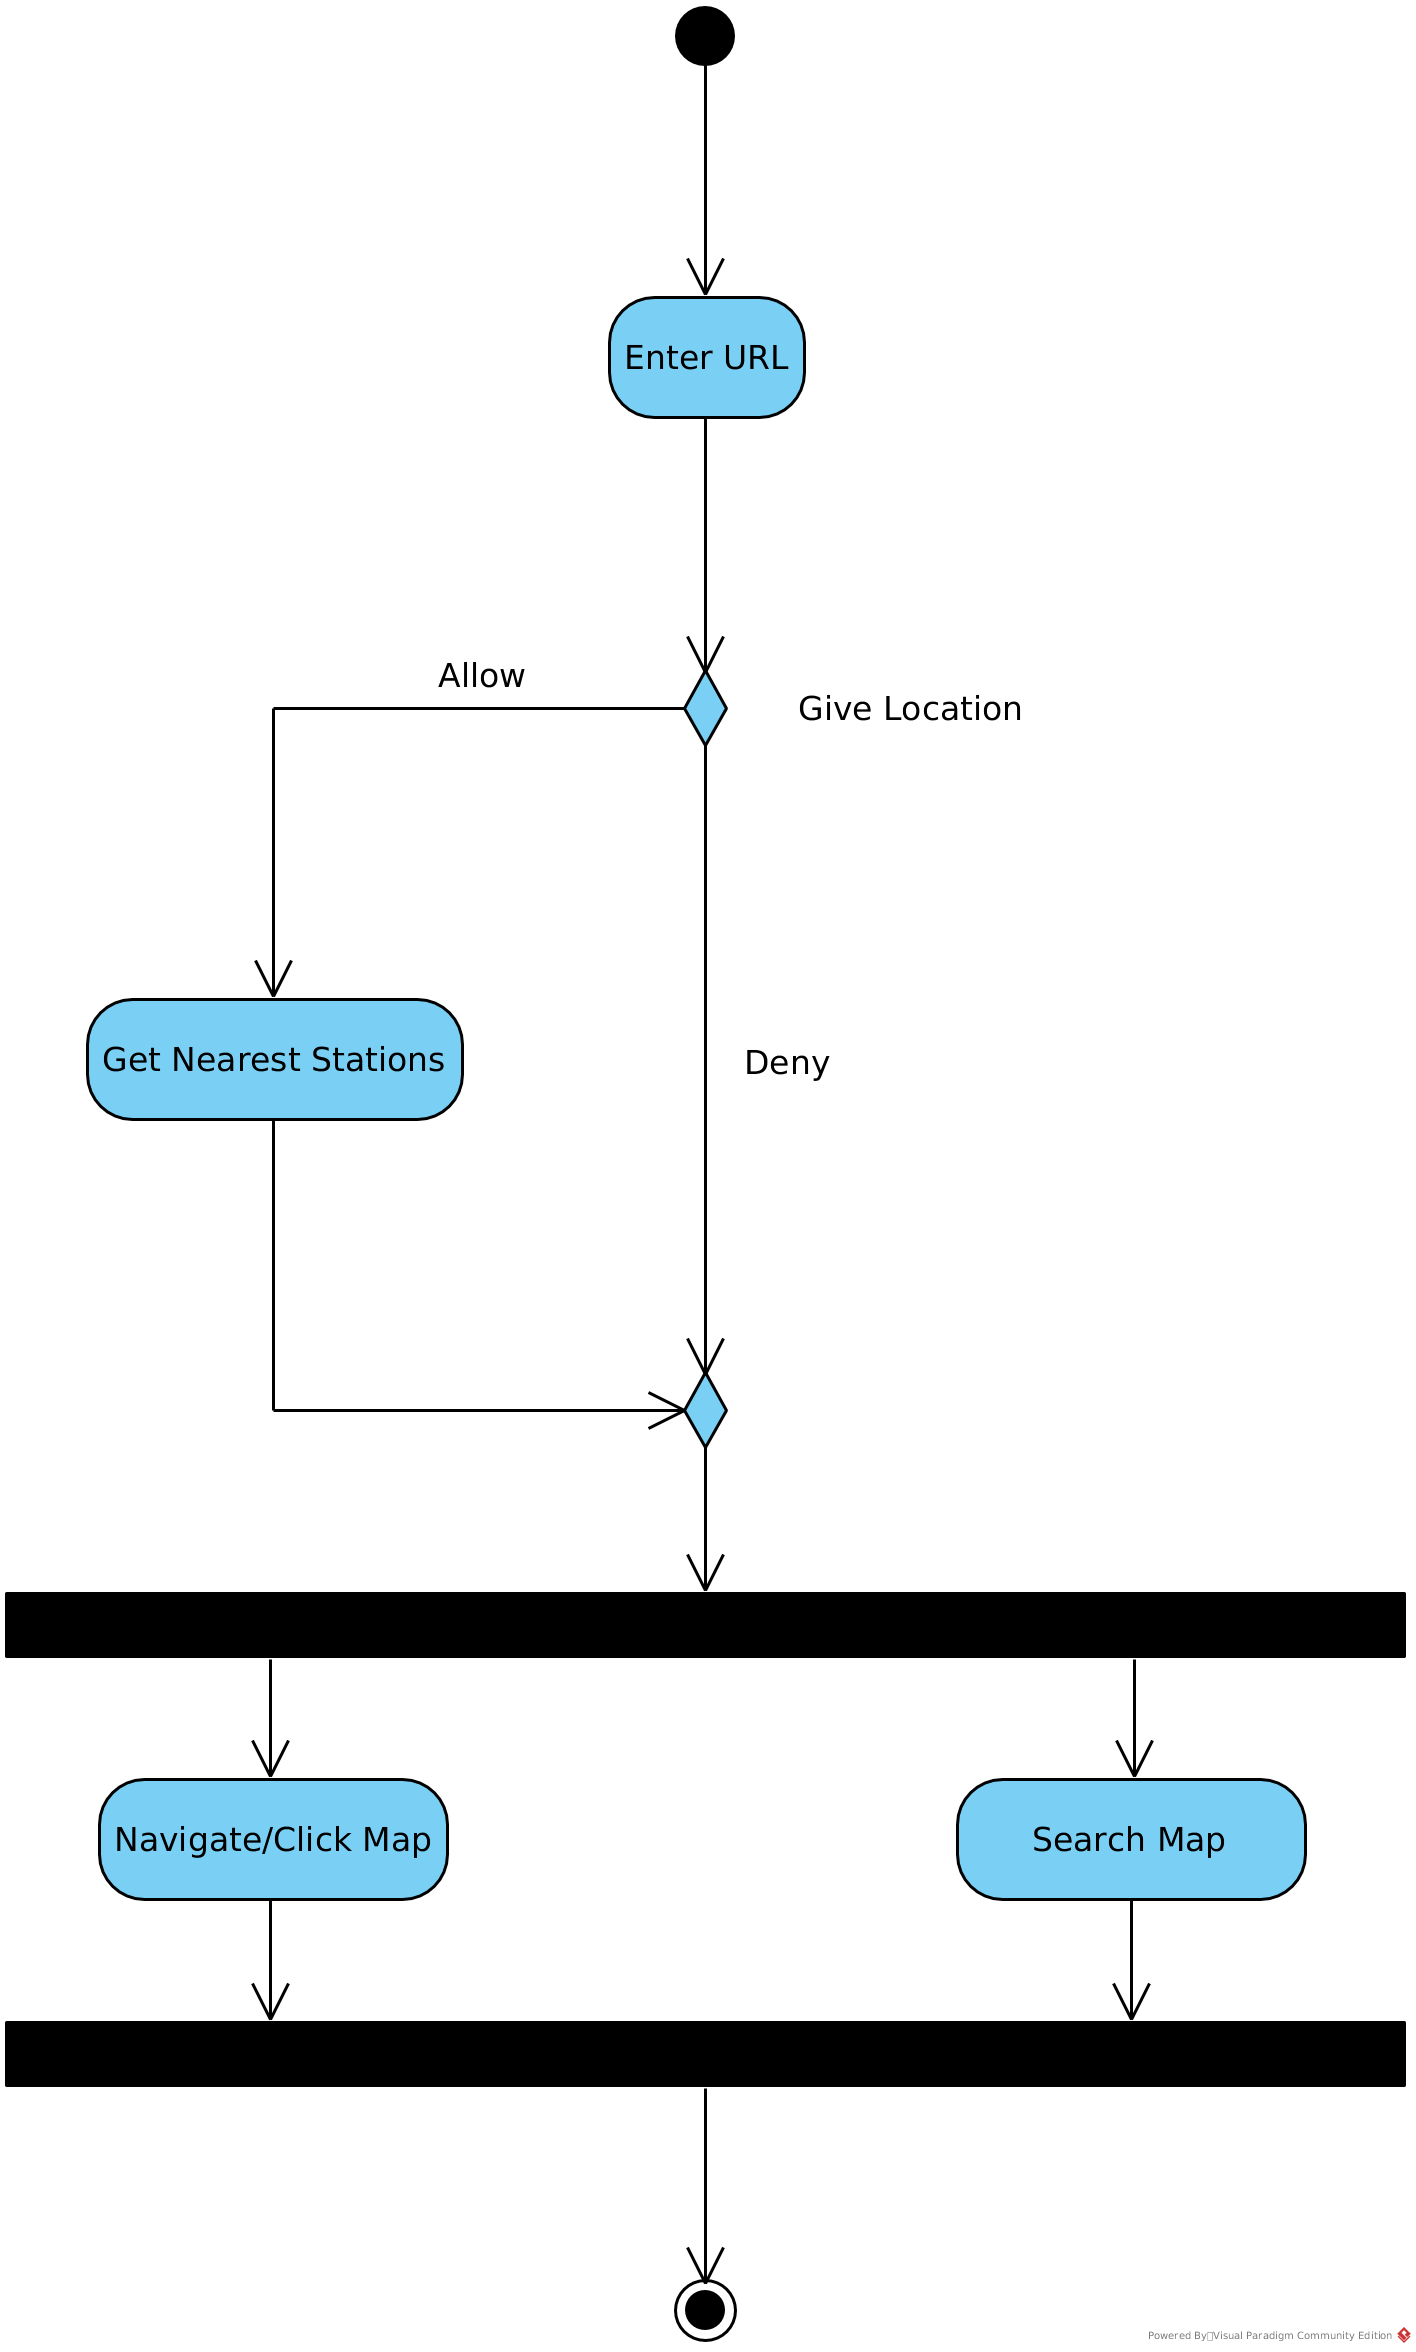
\includegraphics[]{media/Activity/Simple_User.png}
	\caption{Simple User: Activity Diagram}
	\label{fig:Simple_User_Activity}
\end{figure}



\begin{figure}[H]
    \centering
    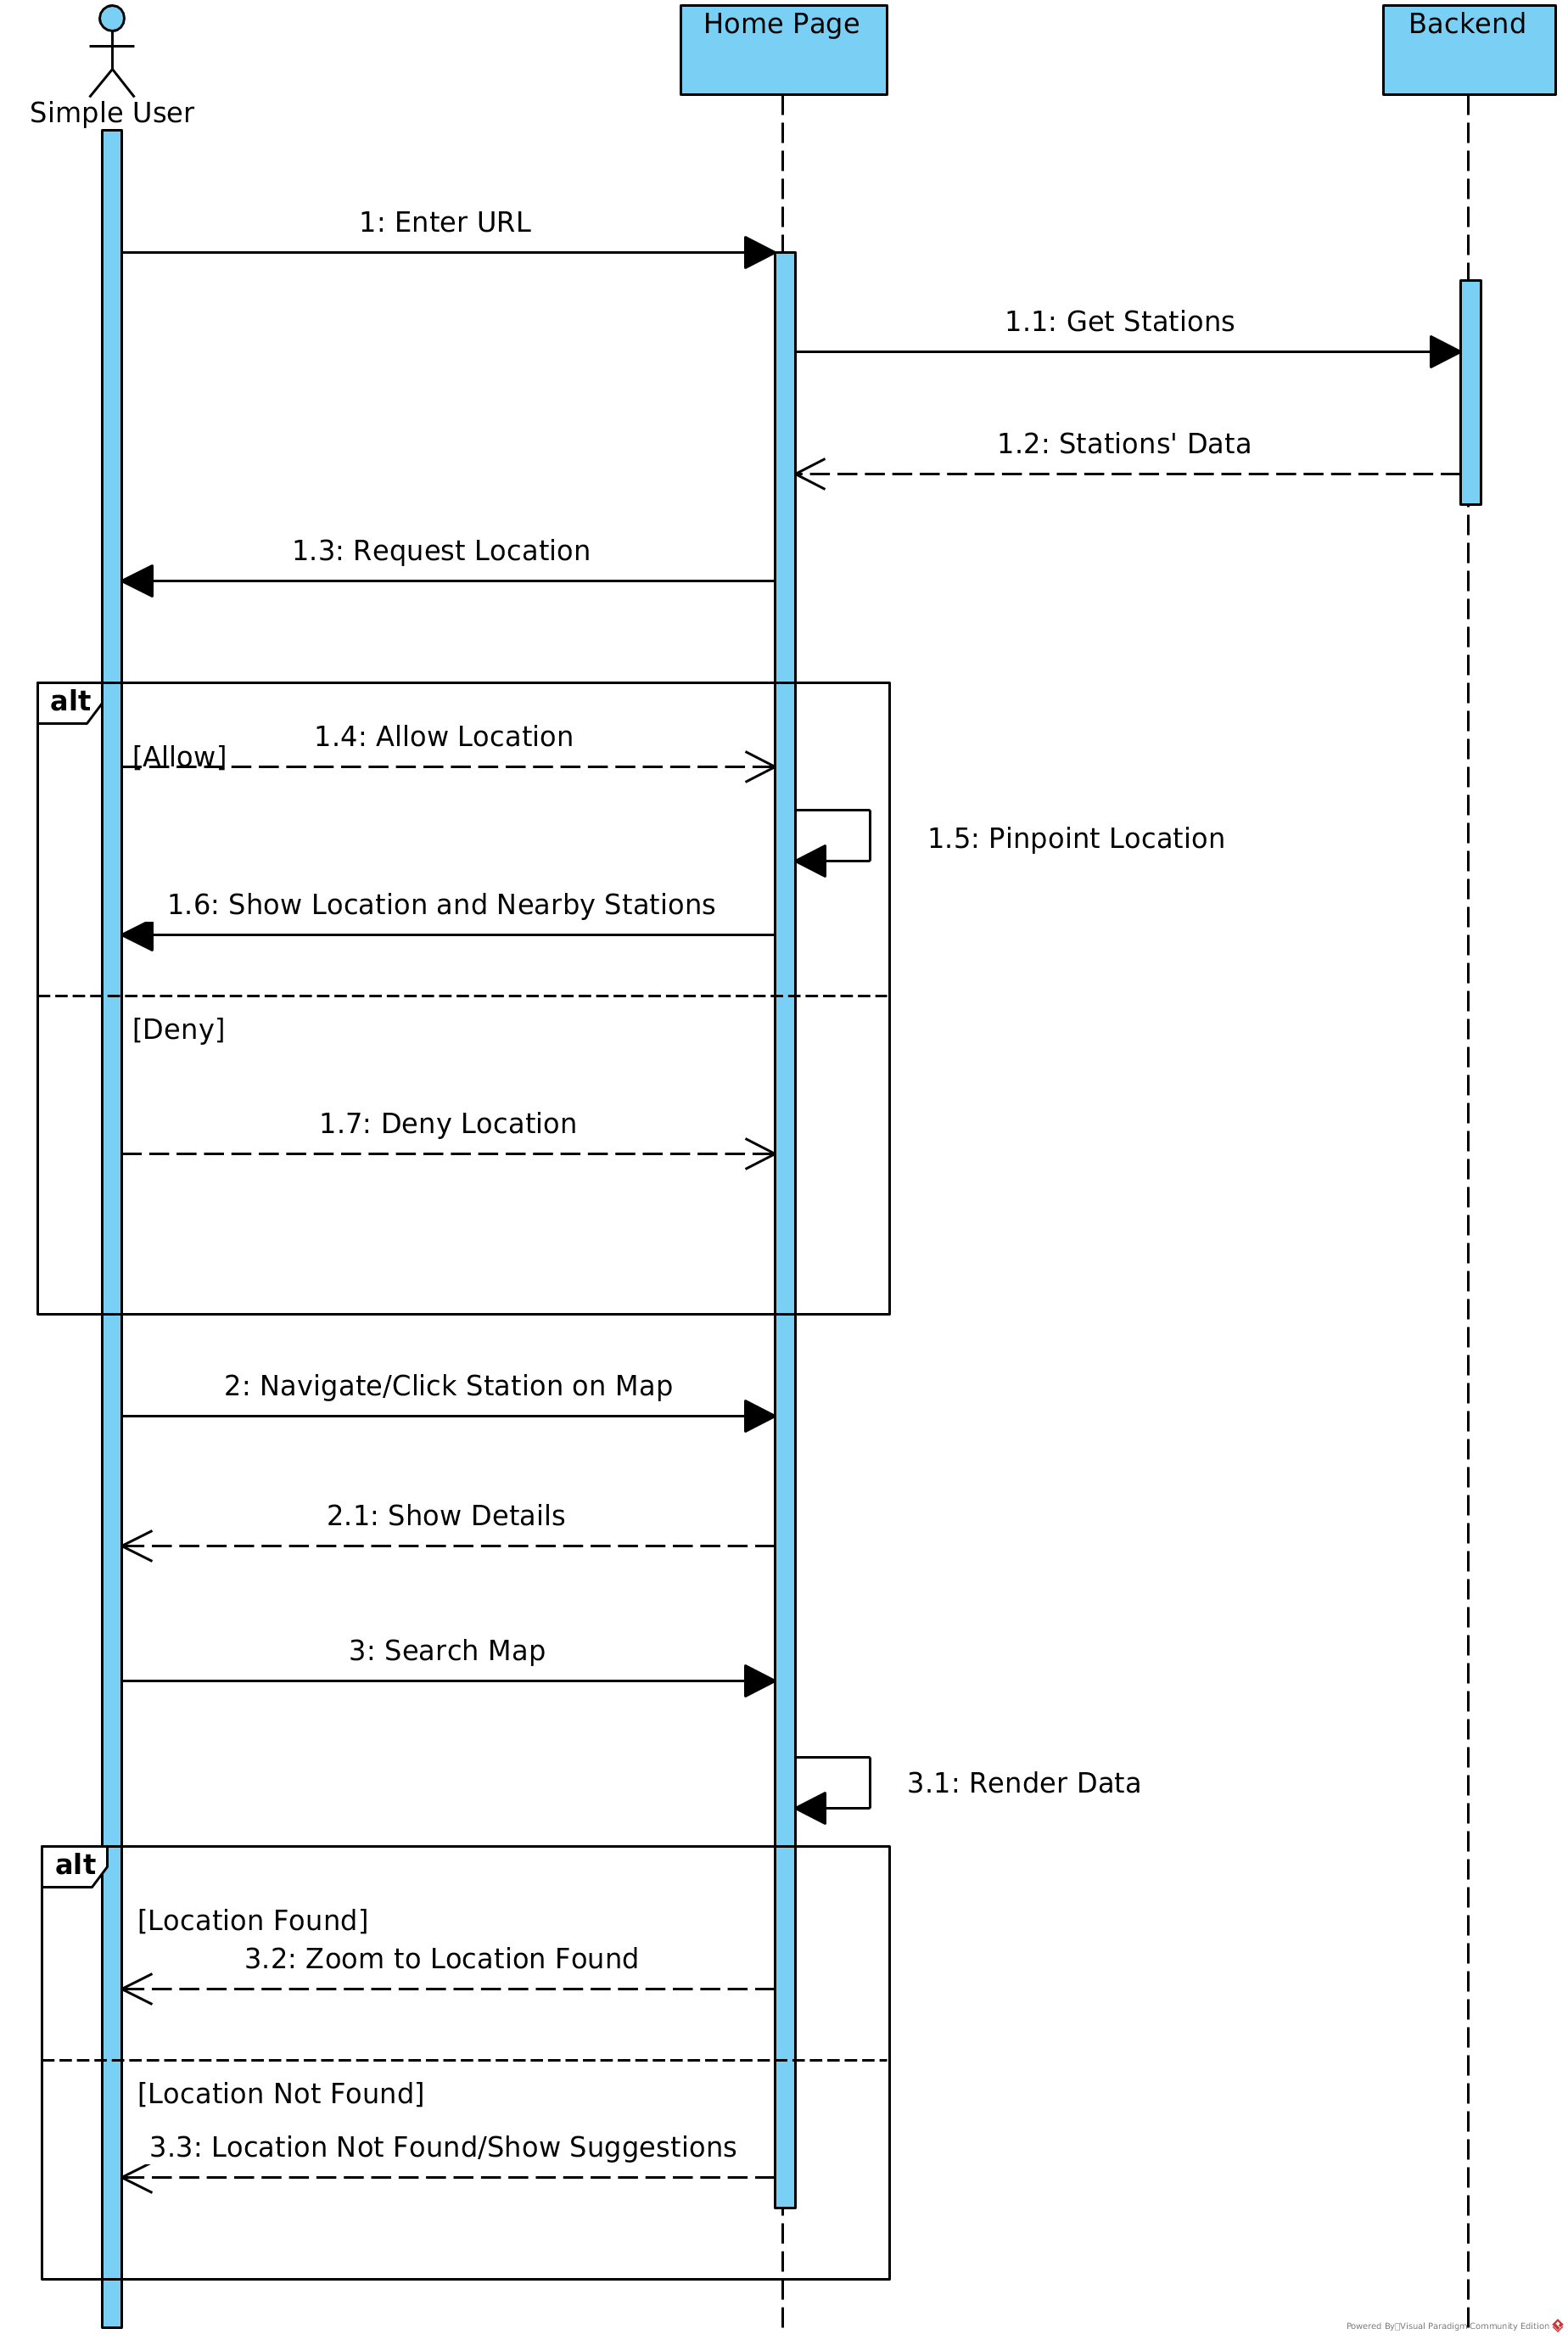
\includegraphics[height=0.9\textheight]{media/Sequence/Simple_User.png}
	\caption{Simple User: Sequence Diagram}
	\label{fig:Simple_User_Sequence}
\end{figure}

